\section{Trouble-Shooting}
\subsection{GNU-Build-System}\label{sec:gnu}
The role of the GNU-Build-System (Figure \ref{fig:GNUBuild}) 
\begin{figure}[h]
	\centering
	
    \psfrag{acinclude.m4}{\textsf{\small acinclude.m4}}
    \psfrag{aclocal.m4}{\textsf{\small aclocal.m4}}
    \psfrag{aclocal}{\textsf{\small aclocal}}
    \psfrag{configure.ac}{\textsf{\small configure.ac}}
    \psfrag{autoconf}{\textsf{\small autoconf}}
    \psfrag{Makefile.am ...}{\textsf{\small Makefile.am}}
    \psfrag{automake}{\textsf{\small automake}}
    \psfrag{libtoolize}{\textsf{\small libtoolize}}
    \psfrag{Makefile.in ...}{\textsf{\small Makefile.in}}
    \psfrag{configure}{\textsf{\small configure}}
    \psfrag{Legende}{\textsf{\small legend}}
    \psfrag{Eingabe-Datei}{\textsf{\small input file}}
    \psfrag{Ausgabe-Datei}{\textsf{\small output file}}
    \psfrag{Programm}{\textsf{\small program}}
    \psfrag{Skript}{\textsf{\small procedure}}
    \psfrag{make}{\textsf{\small make}}
    \psfrag{Makefile ...}{\textsf{\small Makefile}}
  	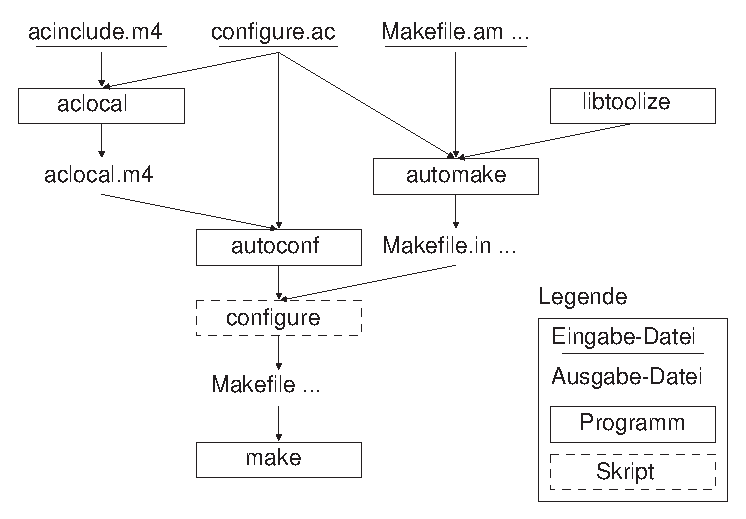
\includegraphics[width=12cm]{Figures/mbsim_gnubuildsystem.eps}
  	\caption{GNU build system}
  	\label{fig:GNUBuild}
\end{figure}
can be summarized as follows.\footnote{in detail: \url{www.gnu.org/software/[autoconf,automake,libtool]/manual}}\par\nopagebreak
	\begin{tabular}{|l|p{100mm}|}
	\hline
		\texttt{aclocal} & Generates M4 macros necessary for the following procedures.\\\hline
		\texttt{autoheader} & Creates \texttt{config.h.in} as basis for header files.\\\hline
		\texttt{autoconf} & Compiler for \texttt{configure.ac} to build the executable \textsc{configure} procedure.\\\hline
		\verb|libtoolize -c --force| & Generates shell and M4 procedures for the system depending shared object files. The option \texttt{-c} forces a local copy of the defining files instead of links. The option \texttt{--force} overwrites already existing procedures.\\\hline
		\texttt{automake -a -c --force} & Compiler for \texttt{Makefile.am} for preparation of \texttt{Makefile.in}. The option \texttt{-c} forces a local copy of the defining files instead of links. The option \texttt{-a} adds missing standard files. The option \texttt{--force} overwrites already existing procedures.\\\hline
		\texttt{autoreconf -fi} & Summarizes \texttt{aclocal}, \texttt{autoheader}, \texttt{autoconf}, \texttt{automake}.\\\hline
		\texttt{make} & Compiles the project sources and links with preliminary libraries. On multi-core computers it is possible to define the number~\texttt{n} of parallel jobs with \texttt{-jn} to accelerate compilation.\\\hline
		\texttt{make install} & Copies the executable project files and \texttt{includes} to \texttt{\$HOME/MBSim/Install}.\\\hline 
        \texttt{./configure} & Invokes system dependent checks and substitutes in existing \texttt{.in}-files variables by systemdepending informationen. The option \texttt{--enable-static --disable-shared} only produces a static build, vice versa a shared library is built. Without such an option normally both shared (*.so) and static (*.a) libraries are provided.\\\hline
	\end{tabular}

\subsection{Third Party Software}\label{sec:third_party}
Necessary for the installation of a static visualisation part are the following preliminary steps with everything being installed by package service or from scratch in \texttt{/home/OpenMBV} with some hints:
\begin{itemize}
\item \texttt{export PKG\_CONFIG\_PATH=/home/OpenMBV/local/lib/pkgconfig}
\item Coin3d with version 3 or newer (3D scenegraphs)\\
    \texttt{./configure --prefix=/home/OpenMBV/local --disable-shared --enable-static}
\item hdf5 with version 1.8.2 or newer (file handling)\\
    \texttt{./configure --prefix=/home/OpenMBV/local --disable-shared --enable-static\\ --enable-cxx --with-zlib=no}
\item Qt with version 4.4 or newer (2D user interface)\\
    \texttt{./configure -prefix /home/OpenMBV/local -static -nomake examples -nomake demos\\ -nomake docs -nomake translations -no-gif -no-libtiff -qt-libpng -no-libmng\\ -qt-libjpeg -no-openssl -no-glib}
\item HDF5Serie (wrapper for file handling)\\
    \texttt{./configure --prefix=/home/OpenMBV/local --disable-shared --enable-static}
\item SoQt with version 1.4.1 or newer (e.g. event invocation in Coin due to hardware events)\\
    \texttt{in SoQtComponent.cpp:103' change "unsinged long key" to "uintptr\_t key"}\\
    \texttt{export QTDIR=/home/OpenMBV/local}\\
    \texttt{export CONFIG\_QTLIBS="\$(pkg-config --libs QtGui QtCore Qt3Support QtOpenGL)"}\\
    \texttt{./configure --prefix=/home/OpenMBV/local --disable-shared --enable-static}
\item Qwt with version 5 or newer (GUI elements)\\
    \texttt{in qwtconfig.pri change INSTALLBASE=/home/OpenMBV/local}\\
    \texttt{/home/OpenMBV/local/bin/qmake}
\item Octave with version 3.0 or newer (for XML preprocessing) 
\end{itemize}

\subsection{Path Information}
After recognising difficulties concerning path information mistakes in the objects should be ruled out by \texttt{make clean}. Then, path information in \texttt{.bashrc} and finally in the affected \texttt{.pc}-files should be checked. The location of the \texttt{.pc}-files can be found by
\begin{verbatim}
pkg-config --cflags mbsim
pkg-config --libs mbsim
\end{verbatim}

\subsection{Often Needed Linux Advices}
\begin{itemize}
\item After editing \texttt{\$HOME/.bashrc} the shell has to be restarted or the command \texttt{source \$HOME/.bashrc} has to be invoked
\end{itemize}

\section{\MBSim{} - Coding Standard}
In the following the Coding standards of \MBSim{} and the associated projects is defined.
\listinginput{1}{mbsimcodingstandard.h}
